\documentclass[a4paper,10pt]{article}
\usepackage{changepage}
\usepackage{xcolor}
\usepackage[T1]{fontenc}
\usepackage{listings}
\usepackage{color}
\usepackage[left=1.5cm, right=2cm, top=1cm, bottom=2cm]{geometry}
\definecolor{dkgreen}{rgb}{0,0.6,0}
\definecolor{gray}{rgb}{0.5,0.5,0.5}
\definecolor{mauve}{rgb}{0.58,0,0.82}

\lstset{frame=tb,
  language=Java,
  aboveskip=3mm,
  belowskip=3mm,
  showstringspaces=false,
  columns=flexible,
  basicstyle={\small\ttfamily},
  numbers=none,
  numberstyle=\tiny\color{gray},
  keywordstyle=\color{blue},
  commentstyle=\color{dkgreen},
  stringstyle=\color{mauve},
  breaklines=true,
  breakatwhitespace=true,
  tabsize=3
}
\renewcommand*\ttdefault{txtt}
\renewcommand*\familydefault{\ttdefault} %% Only if the base font of the document is to be typewriter style
\newcommand{\tbft}[2]{\par\addvspace{\baselineskip}\textbf{#1}\hspace{0.35em}{#2}\\\par\addvspace{\baselineskip}}
\newcommand{\ejercicio}[2]{\par\addvspace{\baselineskip}\textbf{Ejercicio #1.}\hspace{0.35em}{#2}\\\par\addvspace{\baselineskip}}
% \ejercicio{NUMERO}{ENUNCIADO}
%   Devuelve
% Ejercicio NUMERO. ---- ENUNCIADO ----
%
%formato
\newcommand{\salto}[1]{\par\addvspace{#1}}
\newcommand{\rojo}[1]{{\color{red}#1}}
\newcommand{\anotacion}[2][red]{\salto{1ex}\noindent\texttt{\color{#1}#2}\salto{1ex}}
\newcommand{\anotacionns}[2][red]{\noindent\texttt{\color{#1}#2}}
%
% si y solo si corto y largo
\newcommand{\sii}{\leftrightarrow}
\newcommand{\siiLargo}{\longleftrightarrow}
\newcommand{\slr}[1]{\ensuremath{\langle #1\rangle}}
\newcommand{\smm}[1]{\textless #1\textgreater}
\newcommand{\encabezadoTAD}[1]{\par\salto{1ex}\noindent TAD\ \ \normalfont\ttfamily#1 }
\newenvironment{tad}[1]{
\newcommand{\nombretad}{{\ttfamily#1}}
\newcommand{\nt}{\nombretad}
\newcommand{\obs}[2]{\par\noindent{\ttfamily obs} ##1: ##2\par}
\encabezadoTAD{#1}\{
    \begin{adjustwidth}{3em}{0em}}
{\end{adjustwidth}\par\}}
% \begin{tad}{nombre del tad}
%   AGREGAR UN OBSERVADOR
%     \obs{nombre observador}{tipo}
%     \nombretad <---------- DEVUELVE EL NOMBRE DEL TAD (du)
%
%   y aca se pueden usar todos los procs y cosas de la catedra
%
%     \end{tad}
\newcommand{\encabezadoImpl}[3]{\par\salto{1ex}\noindent \textbf{impl}\ \normalfont\ttfamily#1(#2):#3}
\newcommand{\asg}[2]{\salto{0em}\noindent{\ttfamily #1}:= #2\salto{0em}}
\newcommand{\asgns}[2]{\noindent{\ttfamily #1}:= #2}
\newenvironment{impl}[3]{\encabezadoImpl{#1}{#2}{#3}\{
\begin{adjustwidth}{3em}{0em}
}
{\end{adjustwidth}\par\}}
\newcommand{\encabezadoDesign}[2]{\par\salto{1ex}\noindent \textbf{modulo}\ {\normalfont\ttfamily #1} \textbf{implementa}{ \normalfont\ttfamily #2}}
\newenvironment{design}[2]{\encabezadoDesign{#1}{#2}\{
\newcommand{\var}[2]{\salto{0em}\noindent{\normalfont \bfseries var} \texttt{##1}: \texttt{##2}\salto{0em}}
\begin{adjustwidth}{3em}{0em}
}
{\end{adjustwidth}\}}
\newcommand{\ifthel}[3]{\salto{0ex}
\noindent{\normalfont \bfseries if}{ #1 }{\normalfont \bfseries then}\salto{0ex}
\noindent{\begin{adjustwidth}{1.5em}{0em}#2\end{adjustwidth}}\salto{0ex}
\noindent{\normalfont \bfseries else}\begin{adjustwidth}{1.5em}{0em}{#3}\end{adjustwidth}\salto{0ex}
\noindent{\bfseries end if}}\salto{0ex}
\newcommand{\while}[2]{
    \salto{0em}\noindent
    {\normalfont \bfseries while} \ensuremath{#1} \textbf{do}
    \begin{adjustwidth}{1.5em}{0em}{#2}\end{adjustwidth}\salto{0em}\noindent{\normalfont \bfseries end while}
}
\newcommand{\invrep}[2]{\salto{0em}\noindent{\bfseries pred} InvRep (#1)\{\salto{0em}\noindent\begin{adjustwidth}{2em}{0em}{#2}\end{adjustwidth}\salto{0em}\noindent\}}
\newcommand{\abs}[2]{\salto{0em}\noindent{\bfseries pred} Abs (#1)\{\salto{0em}\noindent\begin{adjustwidth}{2em}{0em}{#2}\end{adjustwidth}\salto{0em}\noindent\}}

\usepackage{graphicx}
\usepackage[dvipsnames]{xcolor}
\begin{document}

\paragraph*{Como pensamos representar los elementos:}

\begin{itemize}
    \item $C$: Conjunto de las carreras de grado.


          Lo representamos como Trie que se accede desde la instancia siu.
    \item $c$: Nombre de carrera.


          Lo representamos como string. Por lo tanto |c| indica el largo del nombre de la carrera.
    \item $M_c$: Conjunto de las materias del grado c

          Lo representamos como Trie que se accede desde la instancia de Carrera (Debajo desarrollaremos un ejemplo concreto)
    \item $N_m$: Conjunto de nombres de la materia.

          Los caracteres de estos nombres seran los nodos del Trie anterior. Los nodos significativos apuntaran a las materias respectivas.
    \item $n$: Nombre de la materia

          Lo representamos como un string, por lo tanto |n| indica el largo del nombre de la materia.
    \item $E$ y $E_m$: los representaremos como enterous.
\end{itemize}
\salto{\baselineskip}
Libretas universitarias $\rightarrow$ Trie acotado, lo que implica que las operaciones del trie son de O(1)

{\small El nodo significativo de cada libreta apuntara a la instancia de Estudiante}

\salto{\baselineskip}

NombreCarreras $\rightarrow$ Trie no acotado, operaciones O(log(n))

{\small El nodo significativo apuntara a la instancia de la Carrera}

\salto{\baselineskip}

NombreMaterias $\rightarrow$ Trie no acotado, operaciones O(log(n))

{\small El nodo significativo apuntara a la instancia de Materia}

\salto{\baselineskip}

Veamos el siguiente ejemplo:
\salto{\baselineskip}

Tenemos la carrera fisica y la carrera matematica, en la primera tenemos la materia

"Matematica 1", y en la segunda tenemos 'Analisis 1', ambas siendo la misma materia.

A traves del trie NombreCarreras accedemos a una instancia de la clase Carrera

en el nodo significativo. Esta clase nos permite acceder a su trie NombreMaterias, y en el nodo significativo acceder a la instancia de la materia.



\pagebreak
\vspace*{15ex}
En este caso particular la materia "Matematica 1 / Analisis 1"

es accedida desde dos caminos distintos:
\salto{\baselineskip}
\begin{figure*}[h]
    \centering
    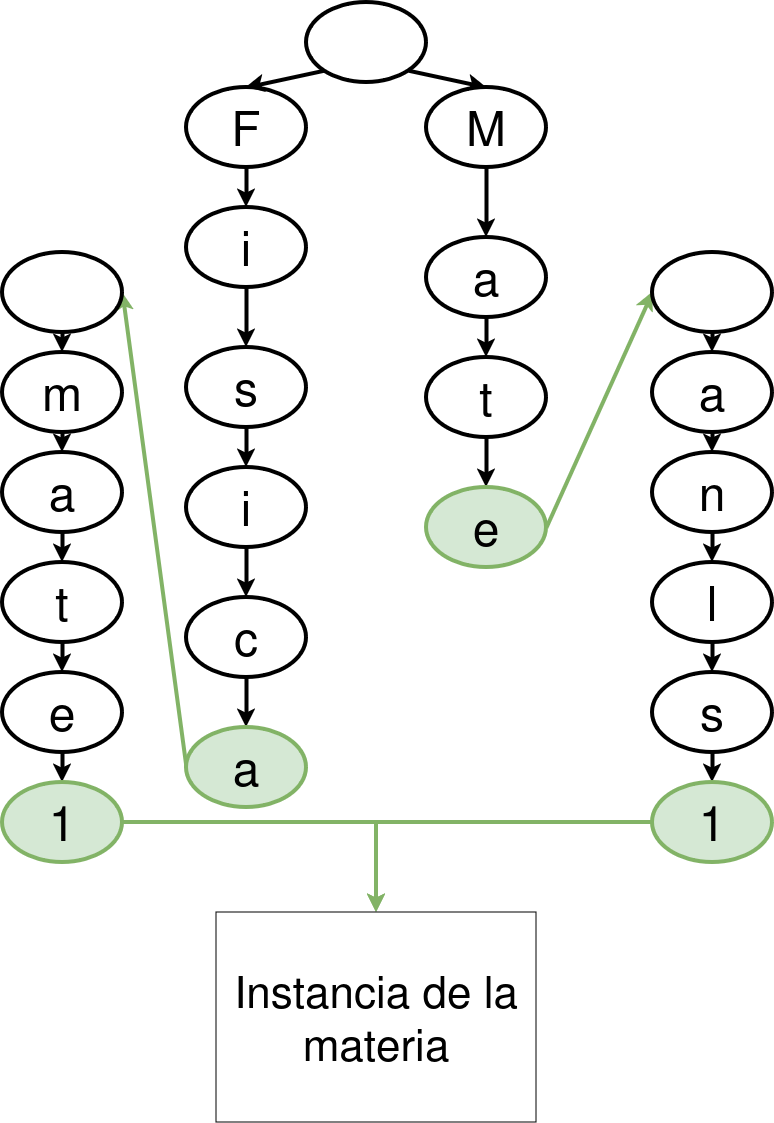
\includegraphics[width=0.5\textwidth]{diagrama1.png}
\end{figure*}
\pagebreak
\section*{Dudas:}
\begin{figure*}[h]
    \centering
    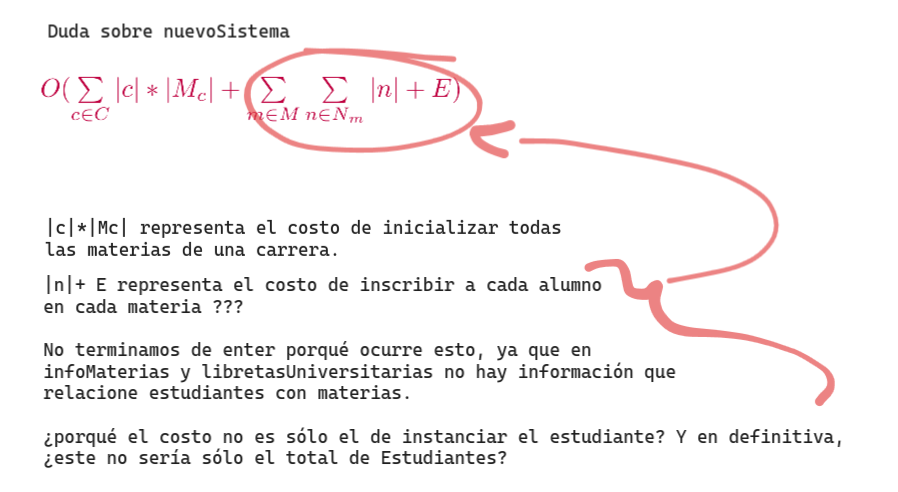
\includegraphics[width=0.7\textwidth]{duda1.png}
\end{figure*}
\pagebreak
\section*{Pseudoresoluciones:}
{\vspace*{-2ex}\hspace*{4em} \small Las que pase a limpio al menos.}


\subsection*{7. carreras(in sistema: SistemaSIU):seq\smm{string}}
\{

\{

    ArrayList lista = new ArrayList() \hfill $\color{Purple}\longleftarrow O(1)$
    
    Iterador it= nuevo iterador del sistemaSIU \hfill $\color{Purple}\longleftarrow O(1)$

    while(iterador.haySiguiente()){\hfill $\color{Purple}\longleftarrow O(\sum_{c\in C}^{} |c|)$

        \hspace*{1.5em} lista.add(iterador.siguiente())

    }

    return lista \hfill $\color{Purple}\longleftarrow O(1)$

\}\hfill $\color{Purple} O(1+1+\sum_{c\in C}^{} |c| +1 )\equiv O(\sum_{c\in C}^{} |c|)$

\noindent\}

\salto{\baselineskip}
\anotacionns[ForestGreen]{Nota: el iterador del trie devuelve los strings ordenador de forma lexicografica.}

\subsection*{8. materias(in sistema: SistemaSIU, in carrera: string):seq\smm{string}}
\{

\{

    Materias materia = Carreras.buscar(carrera) \hfill $\color{Purple}\longleftarrow O(|carrera|)$

    ArrayList lista = new ArrayList() \hfill $\color{Purple}\longleftarrow O(1)$
    
    Iterador it= nuevo iterador del la carrera \hfill $\color{Purple}\longleftarrow O(1)$

    while(iterador.haySiguiente()){\hfill $\color{Purple}\longleftarrow O(\sum_{m_c\in M_c}^{} |m_c|)$

        \hspace*{1.5em} lista.add(iterador.siguiente())

    }

    return lista \hfill $\color{Purple}\longleftarrow O(1)$

\}

\noindent\}\hfill $\color{Purple} O(|carrera|+1+1+\sum_{m_c\in M_c}^{} |m_c| +1 )\equiv O(|carrera|+\sum_{m_c\in M_c}^{} |m_c|)$

\salto{\baselineskip}
\anotacionns[ForestGreen]{Nota: el iterador del trie devuelve los strings ordenador de forma lexicografica.}
\end{document}